\documentclass{ximera}
%%%
\title{TikZ and Tables}
\author{Robert Kelvey, robertkelvey@gmail.com}

\usepackage{multicol}
\usepackage{graphicx}
\usepackage{gnuplottex}
\usepackage[latin1]{inputenc}
\usepackage{tikz}
\usepackage{pgfplots}

\begin{document}

\begin{abstract}
    In this activity, we give drawing a tikZ picture a try and draw some tables.
\end{abstract}

\maketitle

\begin{center}
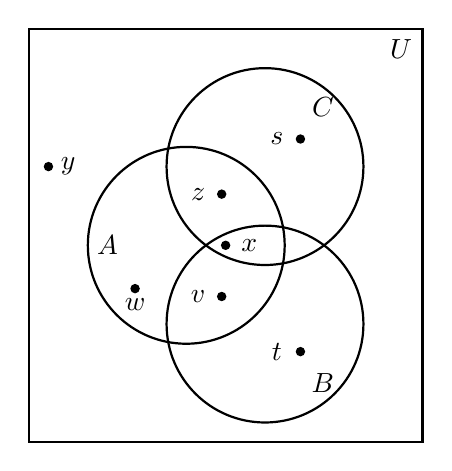
\begin{tikzpicture}
%%%%%DRAW SETS%%%%%%%%%
\draw[thick]  (-2, -2.5) rectangle (3, 2.75) node[below left]{$U$};
\draw[thick] (0,0) circle (1.25cm); 
\draw (-1,0) node {$A$};
\draw[thick] (1,-1) circle (1.25cm); 
\draw (2,-1.75) node[left] {$B$};
\draw[thick] (1,1) circle (1.25cm); 
\draw (2,1.75) node[left] {$C$};

%%%%%DRAW POINTS%%%%%%%
\draw (0.80,0) node {$x$};
\fill[black] (0.50,0) circle (0.06cm); 

\fill[black] (-1.75,1) circle (0.06cm);
\draw (-1.5,1) node {$y$};

\fill[black] (0.45, 0.65) circle (0.06cm);
\draw (0.15,0.65) node {$z$};

\fill[black] (-0.65, -0.55) circle (0.06cm);
\draw (-0.65,-0.75) node {$w$};

\fill[black] (0.45, -0.65) circle (0.06cm);
\draw (0.15,-0.65) node {$v$};

\fill[black] (1.45, -1.35) circle (0.06cm);
\draw (1.15,-1.35) node {$t$};

\fill[black] (1.45, 1.35) circle (0.06cm);
\draw (1.15,1.35) node {$s$};

\end{tikzpicture}
\end{center}

\begin{question}
Identify the following as true or false using the universal set $U$ above and its subsets $A$, $B$, and $C$. \\ Enter your answers with a `T' for true or `F' for false.
    \begin{enumerate}
        \item $v \in A \cap C  \answer[given]{F}$
			
			\item $y \in \bar{A} \cap \bar{B} \cap \bar{C}  \answer{T}$
			
			\item $x \in A - B \answer{F} $
			
			\item $z \in (A \cup C) \cap B  \answer{F}$
			
			\item $\emptyset \subseteq C \answer{T}$
			
			\item $\{w, s, z\} \subseteq (A - C) \cup (C - A) \answer{F}$
			
			\item $\{y,t\} \subseteq \bar{B} \cup \bar{C} \answer{T}$
			
			\item $\{s\} \in \mathcal{P}(C) \answer{T}$
    \end{enumerate}

\end{question}

The above did not use multicols, nor was there a use of the ``prompt" command. We try both below to see what will happen!

\begin{question}
Identify the following as true or false using the universal set $U$ above and its subsets $A$, $B$, and $C$. \\ Enter your answers with a 'T' for true or 'F' for false.
\begin{prompt}
    \begin{enumerate}
    \begin{multicols}{2}

        \item $v \in A \cap C  \answer[given]{F}$
			
			\item $y \in \bar{A} \cap \bar{B} \cap \bar{C}  \answer{T}$
			
			\item $x \in A - B \answer{F} $
			
			\item $z \in (A \cup C) \cap B  \answer{F}$
			
			\item $\emptyset \subseteq C \answer{T}$
			
			\item $\{w, s, z\} \subseteq (A - C) \cup (C - A) \answer{F}$
			
			\item $\{y,t\} \subseteq \bar{B} \cup \bar{C} \answer{T}$
			
			\item $\{s\} \in \mathcal{P}(C) \answer{T}$
    \end{multicols}
    \end{enumerate}
\end{prompt}
\end{question}

In the above, we had the first answer with the ``given" option. Now we list all answers as ``given" in the remixed question below.
\begin{question}
Identify the following as true or false using the universal set $U$ above and its subsets $A$, $B$, and $C$. \\ Enter your answers with a 'T' for true or 'F' for false.
\begin{prompt}
    \begin{enumerate}
    \begin{multicols}{2}

        \item $v \in A \cap C  \answer[given]{F}$
			
			\item $y \in \bar{A} \cap \bar{B} \cap \bar{C}  \answer[given]{T}$
			
			\item $x \in A - B \answer[given]{F} $
			
			\item $z \in (A \cup C) \cap B  \answer[given]{F}$
			
			\item $\emptyset \subseteq C \answer[given]{T}$
			
			\item $\{w, s, z\} \subseteq (A - C) \cup (C - A) \answer[given]{F}$
			
			\item $\{y,t\} \subseteq \bar{B} \cup \bar{C} \answer[given]{T}$
			
			\item $\{s\} \in \mathcal{P}(C) \answer[given]{T}$
    \end{multicols}
    \end{enumerate}
\end{prompt}
\end{question}

Now we try the above but without the single answer prompt. Instead, we employ a multiple choice for each item, with two choices: `T' or `F'.

\begin{question}  
Identify the following as true or false using the universal set $U$ above and its subsets $A$, $B$, and $C$.
\begin{prompt}
\begin{enumerate}
    \begin{multicols}{2}
        \item $v \in A \cap C$
            \begin{multipleChoice}
			    \choice{T}
                \choice[correct]{F}
            \end{multipleChoice} 
			
		\item $y \in \bar{A} \cap \bar{B} \cap \bar{C}$
		    \begin{multipleChoice}
			    \choice[correct]{T}
                \choice{F}
            \end{multipleChoice}	
		\item $x \in A - B$
		    \begin{multipleChoice}
			    \choice{T}
                \choice[correct]{F}
            \end{multipleChoice}	
		\item $z \in (A \cup C) \cap B$
		    \begin{multipleChoice}
			    \choice{T}
                \choice[correct]{F}
            \end{multipleChoice}	
		\item $\emptyset \subseteq C$
		    \begin{multipleChoice}
			    \choice[correct]{T}
                \choice{F}
            \end{multipleChoice}	
		\item $\{w, s, z\} \subseteq (A - C) \cup (C - A)$
		    \begin{multipleChoice}
			    \choice{T}
                \choice[correct]{F}
            \end{multipleChoice}	
		\item $\{y,t\} \subseteq \bar{B} \cup \bar{C}$
		    \begin{multipleChoice}
			    \choice[correct]{T}
                \choice{F}
            \end{multipleChoice}	
		\item $\{s\} \in \mathcal{P}(C)$
	        \begin{multipleChoice}
			    \choice[correct]{T}
                \choice{F}
            \end{multipleChoice}
		\end{multicols} 
\end{enumerate}
\end{prompt}
\end{question}

OKAY so it looks like multiple choice does not like multicols very much. Let's try that again, but without multicols.

\begin{question}  
Identify the following as true or false using the universal set $U$ above and its subsets $A$, $B$, and $C$.
\begin{prompt}
\begin{enumerate}
        \item $v \in A \cap C$
            \begin{multipleChoice}
			    \choice{T}
                \choice[correct]{F}
            \end{multipleChoice} 
			
		\item $y \in \bar{A} \cap \bar{B} \cap \bar{C}$
		    \begin{multipleChoice}
			    \choice[correct]{T}
                \choice{F}
            \end{multipleChoice}	
		\item $x \in A - B$
		    \begin{multipleChoice}
			    \choice{T}
                \choice[correct]{F}
            \end{multipleChoice}	
		\item $z \in (A \cup C) \cap B$
		    \begin{multipleChoice}
			    \choice{T}
                \choice[correct]{F}
            \end{multipleChoice}	
		\item $\emptyset \subseteq C$
		    \begin{multipleChoice}
			    \choice[correct]{T}
                \choice{F}
            \end{multipleChoice}	
		\item $\{w, s, z\} \subseteq (A - C) \cup (C - A)$
		    \begin{multipleChoice}
			    \choice{T}
                \choice[correct]{F}
            \end{multipleChoice}	
		\item $\{y,t\} \subseteq \bar{B} \cup \bar{C}$
		    \begin{multipleChoice}
			    \choice[correct]{T}
                \choice{F}
            \end{multipleChoice}	
		\item $\{s\} \in \mathcal{P}(C)$
	        \begin{multipleChoice}
			    \choice[correct]{T}
                \choice{F}
            \end{multipleChoice}
\end{enumerate}
\end{prompt}
\end{question}

That seems to look better.

Now we will try...



\end{document}
